\chapter{不変な法則、四元ベクトル、場のテンソル}

まず、自然が従ってもよかったのに従っていない法則から始めよう。その失敗は、物理法則がどのように書かれるべきかを教えてくれる。同じ試練は、まず座標成分から通常のベクトルへ、次に通常のベクトルから四元ベクトルへ、最後に四元ベクトルからテンソルへと導く。最終的には、電場と磁場はもはや別々の対象ではなくなる。それらは共に、一つの反対称テンソルの6つの独立な枠を占めるのである。

特に断らない限り、\(c=1\) とする単位系を用い、時空成分を \((1,2,3,0)=(x,y,z,t)\) の順に並べ、計量の符号を \((-,-,-,+)\) とする。

\section{誤った対称性をもつ可能な法則}

空間に \(x\) 軸と \(y\) 軸を永久に固定する。次に、二つの粒子の \(x\) 座標が一致するときはいつでも相互作用すると定めよう。相互作用はそれらの運動を逆転させるかもしれないし、新しい方向へと送り出すかもしれない。その詳細な力学は問題ではない。提案された引き金は単に
\begin{equation}
  x_1-x_2=0,
\end{equation}
である。ここで添字は座標成分ではなく粒子を表す。この規則には数学的矛盾はない。問題は、何がこれを物理的にありそうにないものにするのかである。

\begin{classroomqa}
\audiencequestion{この規則は空間の一様性に反するか。}
\lecturerresponse{反しない。原点を平行移動すると両方の座標が同じ量だけ変わり、\(x_1-x_2\) は変わらない。この規則は特別な場所を指定していない。その欠陥は等方性である。すなわち、一つの特別な方向を選び出している。}
\end{classroomqa}

軸を \(90^\circ\) 回転させる。古い \(x\) 方向は今や \(y\) と呼ばれるので、同じ物理的出来事は \(y\) 座標の等しさによって記述されることになる。一般の角度では、条件は \(x\) と \(y\) の線形結合を含むことになる。したがって、法則の形は黒板がどのように向けられていたかに依存する。それは平行移動不変であるが、回転不変ではない。

通常、物理法則は直交座標において最も簡単な形で与えられる。より一般の座標を用いてもよいが、その場合には計量と公式はより簡単でなくなる。直交デカルト系の範囲内では、いかなる向きも特権的であってはならない。

修正は即座である。二次元では両方の座標が一致することを要求し、三次元では三つすべてが一致することを要求する。
\begin{equation}
  x_1=x_2,
  \qquad y_1=y_2,
  \qquad z_1=z_2.
\end{equation}
そのとき粒子は、たとえ異なる直線に沿って近づいても、同じ点に到達したときにのみ相互作用できる。

\begin{classroomqa}
\audiencequestion{\(z\) 座標と時間も一致しなければならないか。}
\lecturerresponse{三次元空間では \(z\) 座標も一致しなければならない。時間は今のところ抑えている。空間についての議論が完了し次第、復元される。}
\end{classroomqa}

\(\boldsymbol r_a\) を粒子 \(a\) の位置とする。三つの成分条件は一つのベクトル方程式になる。
\begin{equation}
  \boldsymbol r_1-\boldsymbol r_2=\boldsymbol 0.
\end{equation}
成分はある回転された系では消え、別の系では消えないかもしれない。ベクトル全体は異なる。ある系で全ての成分がゼロならば、どの回転された系でも全ての成分がゼロである。同様に、二つのベクトルがある系で等しければ、両方を変換した後でも等しいままである。

\begin{figure}[H]
\centering
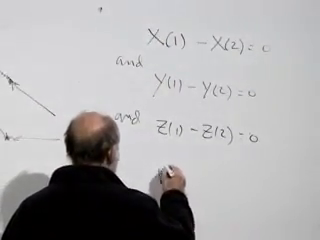
\includegraphics[width=0.78\textwidth]{lecture_06_figure_01.png}
\caption{衝突が一つの特権的な軸に沿った一致ではなく空間的な同時位置を意味するようにする三つの座標の等しさ。}
\lectureframe{00:09:00}
\end{figure}

これがベクトル方程式が有用である理由である。その成分は変化するが、対象は首尾一貫して変換する。完全な対象について書かれた法則は、座標が回転されてもその形を保つことができる。

\section{時空における同時位置}

次に、垂直な空間軸を時間で置き換える。ニュートン的な規則では、二つの運動の変化は等しい時間にのみ起こると言うかもしれない。ニュートン力学では同時性はすべての慣性観測者に共有されるので、そのような規則は可能である。特殊相対性理論では、それは特権的な系を選び出す。ある系で同時である出来事は、別の系でも同時である必要はない。

空間座標のみの等しさを要求するのも同様に良くない。時空変位は空間成分がゼロで時間成分が非ゼロでありうる。
\begin{equation}
  \Delta X^\mu=(0,0,0,\Delta t),
\end{equation}
そしてブーストは \(\Delta t\) を空間成分と混合する。不変な局所的言明は、二つの運動の変化が同じ事象で起こるということである。したがって、単純な衝突は次を要求する。
\begin{equation}
  X_1^\mu=X_2^\mu,
  \qquad\text{or}\qquad
  X_1^\mu-X_2^\mu=0.
\end{equation}
四つの座標すべてが一致する。すなわち、粒子は同じ時刻に同じ場所を占める。

衝突の例は、物理学を書くための一般的な規則を与える。すべてを一方の側に置いて完全な四元ベクトルをゼロに等しいと置くか、あるいは一つの完全な四元ベクトルを別のものに等しいと置けばよい。四元ベクトルの無関係な部分を等置することは、それ自体ではローレンツ不変な言明を与えない。

\section{ブースト、回転、行列記法}

4元ベクトルとは、時空変位と同じように変換する対象である。この定義を有用なものにするために、まず座標そのものの変換を思い出そう。\(x\)方向の速さ\(v\)のブーストに対して、
\begin{align}
  x'&=\gamma(x-vt), & y'&=y, & z'&=z,
  & t'&=\gamma(t-vx),                                      \label{eq:l6-boost}
\end{align}
ここで
\begin{equation}
  \gamma(v)=\frac{1}{\sqrt{1-v^2}}.
\end{equation}

\begin{classroomqa}
\audiencequestion{これらの式では光速が1に等しいと置かれているのか。}
\lecturerresponse{はい。単位を復元するには、\(X^0=ct\)とし、\(1-v^2\)を\(1-v^2/c^2\)に置き換え、混合した空間--時間の項に対応する\(c\)の因子を復元すればよい。}
\end{classroomqa}

\(z\)軸まわりの回転は\(x\)と\(y\)を混合し、\(z\)と\(t\)はそのままにする：
\begin{equation}
\begin{pmatrix}
  x'\\ y'\\ z'\\ t'
\end{pmatrix}
=
\begin{pmatrix}
  \cos\theta & \sin\theta & 0 & 0\\
  -\sin\theta & \cos\theta & 0 & 0\\
  0 & 0 & 1 & 0\\
  0 & 0 & 0 & 1
\end{pmatrix}
\begin{pmatrix}
  x\\ y\\ z\\ t
\end{pmatrix}.
\end{equation}
ゼロは表示する価値がある。それらは、与えられた変換後の座標にどの成分が入らないかを明示的に示している。同じ順序で、式~\eqref{eq:l6-boost}のブーストは
\begin{equation}
\begin{pmatrix}
  x'\\ y'\\ z'\\ t'
\end{pmatrix}
=
\begin{pmatrix}
  \gamma & 0 & 0 & -\gamma v\\
  0 & 1 & 0 & 0\\
  0 & 0 & 1 & 0\\
  -\gamma v & 0 & 0 & \gamma
\end{pmatrix}
\begin{pmatrix}
  x\\ y\\ z\\ t
\end{pmatrix}.
\end{equation}

回転とブーストは行列の積によって合成できる。元の\(x\)軸と一致しない方向にブーストするには、その方向を\(x\)軸へ回転し、ブーストを適用し、必要に応じて回転すればよい。これら基本行列の積は、より一般的なローレンツ変換を生成する。

\begin{classroomqa}
\audiencequestion{先に回転してからブーストするか、先にブーストしてから回転するかは重要か。}
\lecturerresponse{はい。最初の操作の後では、2番目の操作が作用する軸が変わっている。2つの行列の積は一致する必要がないので、操作の順序が重要である。}
\end{classroomqa}

これらすべての線形変換は一度に
\begin{equation}
  X'^{\mu}=\Lambda^{\mu}{}_{\nu}X^{\nu}.                  \label{eq:l6-vector-transform}
\end{equation}
と書ける。繰り返された添字\(\nu\)は\(1,2,3,0\)について和をとる。これは行列の積における通常の行ごとの列和を、添字記法で表したものにすぎない。

\begin{figure}[H]
\centering
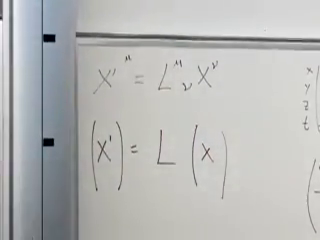
\includegraphics[width=0.78\textwidth]{lecture_06_figure_02.png}
\caption{その列ベクトル形式の冒頭より上の添字付きローレンツ変換。}
\lectureframe{00:31:55}
\end{figure}

式~\eqref{eq:l6-vector-transform}は一般の反変4元ベクトルの定義でもある。\(A^\mu\)がそのようなベクトルならば、
\begin{equation}
  A'^{\mu}=\Lambda^{\mu}{}_{\nu}A^{\nu}.
\end{equation}
その4つの成分は位置を表す必要はない。その対象を4元ベクトルにするのは、その変換則である。

\section{スカラー、計量、不変な積}

さらに4元ベクトルを使う前に、より単純なスカラーの概念に立ち返ると役に立つ。空間回転の下で、指定された点における温度はスカラーであり、指定された2点間の距離も同様である。どちらも1つの数であり、軸の向きに依存しない。センチメートルで測った距離が華氏度で測った室温に等しいという、わざとばかげた数値的主張をすることさえできる。この主張には物理的な深みはないが、両辺が回転スカラーであるため、その真偽は軸をどのように回しても依存しない。

ベクトルの成分はスカラーではない。したがって、それらをスカラーに組み合わせる体系的な方法が必要である。一般の反変4元ベクトルを
\begin{equation}
  A^\mu=(A^1,A^2,A^3,A^0).
\end{equation}
と書く。共変成分は、同じ幾何学的対象を下付き添字で表す。我々の符号では、それらはミンコフスキー計量を用いて得られ、
\begin{equation}
  A_\mu=\eta_{\mu\nu}A^\nu,
  \qquad
  \eta_{\mu\nu}=
  \begin{pmatrix}
    -1&0&0&0\\
    0&-1&0&0\\
    0&0&-1&0\\
    0&0&0&1
  \end{pmatrix},                                          \label{eq:l6-metric}
\end{equation}
したがって
\begin{equation}
  A_\mu=(-A^1,-A^2,-A^3,A^0).
\end{equation}

\begin{classroomqa}
\audiencequestion{ボード上の2つの添字と符号は矛盾しているのか。}
\lecturerresponse{はい。表示された列の空間成分には対応する負号が必要であり、添字下げの式の右辺の成分は\(\eta_{\mu\nu}\)を掛ける前に上付き添字を持つ。時間のラベルは\(4\)ではなく\(0\)である。}
\end{classroomqa}

\begin{figure}[H]
\centering
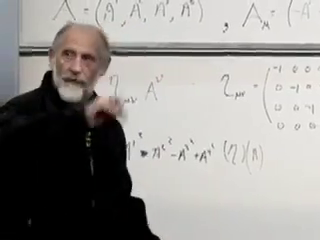
\includegraphics[width=0.8\textwidth]{lecture_06_figure_03.png}
\caption{反変成分と共変成分、計量行列、そして不変な縮約の冒頭。}
\lectureframe{00:45:00}
\end{figure}

添字下げは飾りではない。それはローレンツ不変なノルムに必要な符号をまとめる：
\begin{align}
  A_\mu A^\mu
  &=-(A^1)^2-(A^2)^2-(A^3)^2+(A^0)^2,                    \label{eq:l6-norm}\\
  X_\mu X^\mu
  &=t^2-x^2-y^2-z^2.
\end{align}
2番目の式は原点からの不変な時空間隔である。\(A^\mu\)は\(X^\mu\)と同じように変換するので、その縮約も同じ不変性を持つ。

この記法はまた、有用な勘定規則を教えてくれる。繰り返される総和添字は上付きに一度、下付きに一度現れる。例えば、
\begin{equation}
  A_\mu A^\mu
  =\eta_{\mu\nu}A^\mu A^\nu.
\end{equation}
総和される添字、すなわちダミー添字の名前は、その量を変えることなく変更してよい。

\begin{classroomqa}
\audiencequestion{これらのベクトルの一方を行、他方を列と見なすべきか、またそれらの順序は重要か。}
\lecturerresponse{現在の計算では、添字付きの量を成分と見なし、計量に縮約を行わせればよい。議論を行対列の演算子代数に変える必要はない。これらは通常の数なので、その順序は重要ではない。非可換な演算子ならばより注意が必要だが、それはここでの主題ではない。}
\end{classroomqa}

同じ構成により、異なる二つの四元ベクトルの間の内積が得られる。
\begin{equation}
  A\mathbin{\cdot}B=A_\mu B^\mu=A^\mu B_\mu.
\end{equation}
その不変性は、ローレンツ行列を陽に書くことなく従う。\(A+B\) と \(A-B\) は四元ベクトルであるから、それらのノルムの二乗はいずれも不変である：
\begin{align}
  (A+B)^2&=A^2+B^2+2A\mathbin{\cdot}B,\\
  (A-B)^2&=A^2+B^2-2A\mathbin{\cdot}B.
\end{align}
差を取ると
\begin{equation}
  (A+B)^2-(A-B)^2=4A\mathbin{\cdot}B,                    \label{eq:l6-polarization}
\end{equation}
したがって \(A\mathbin{\cdot}B\) もまた不変である。因子の4は展開から直接に従う。\editorialnote{黒板での議論がこの偏極恒等式を与える。因子を書き下すことで、口頭での相殺が曖昧でなくなる。}

\begin{figure}[H]
\centering
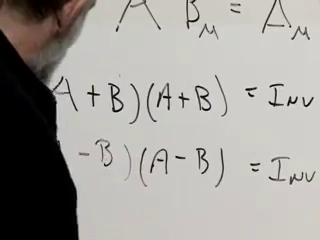
\includegraphics[width=0.8\textwidth]{lecture_06_figure_04.png}
\caption{異なる四元ベクトルの内積を分離するために用いられた二つの不変な平方。}
\lectureframe{00:52:20}
\end{figure}

不変量は物理法則の自然な構成要素である。孤立した成分と異なり、それらは座標系から座標系へと同じ値をもたらす。

\section{固有速度と四元運動量}

粒子の世界線上の隣接する二つの事象を考える。それらの隔たりは無限小四元ベクトル
\begin{equation}
  dX^\mu=(dx,dy,dz,dt).
\end{equation}
である。時間的 worldline に対して、固有時間は
\begin{equation}
  d\tau^2=dX_\mu dX^\mu
  =dt^2-dx^2-dy^2-dz^2.                                  \label{eq:l6-proper-time}
\end{equation}
により定義される。固有四元速度は
\begin{equation}
  U^\mu=\frac{dX^\mu}{d\tau}.                            \label{eq:l6-four-velocity}
\end{equation}
であり、これは選ばれた座標系の座標時間ではなく、粒子自身の固有時間に関する時空位置の変化率を測る。

\(U^\mu\) は4つの成分をもつが、独立なのは3つだけである。式~\eqref{eq:l6-proper-time} を \(d\tau^2\) で割ると
\begin{equation}
  U_\mu U^\mu=1.
\end{equation}
が得られる。したがって四元速度は単位時間的ベクトルである。未来向きの選択がその時間成分の符号を定める。

\begin{classroomqa}
\audiencequestion{\(c\) よりずっと小さい速さでは、四元速度は通常の速度に帰着するか。}
\lecturerresponse{その3つの空間成分は通常の速度に近づき、時間成分は \(c=1\) 単位で1に近づく。この関係は連鎖律を適用し \(dt/d\tau\) を計算することから従う。}
\end{classroomqa}

各空間成分について、
\begin{equation}
  U^i=\frac{dx^i}{d\tau}
     =\frac{dx^i}{dt}\frac{dt}{d\tau}
     =v^i\frac{dt}{d\tau}.
\end{equation}
式~\eqref{eq:l6-proper-time} を \(dt^2\) で割る：
\begin{equation}
  \left(\frac{d\tau}{dt}\right)^2
  =1-v_x^2-v_y^2-v_z^2
  =1-\boldsymbol v^2.
\end{equation}
したがって
\begin{equation}
  \frac{dt}{d\tau}=\frac{1}{\sqrt{1-\boldsymbol v^2}}
  =\gamma(\lvert\boldsymbol v\rvert),
\end{equation}
であり、
\begin{equation}
  U^\mu=(\gamma v_x,\gamma v_y,\gamma v_z,\gamma).
                                                                  \label{eq:l6-u-components}
\end{equation}

\begin{figure}[H]
\centering
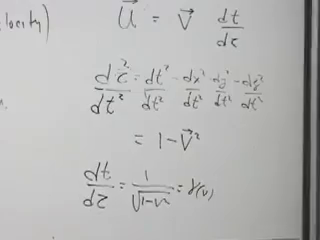
\includegraphics[width=0.8\textwidth]{lecture_06_figure_05.png}
\caption{\(dt/d\tau=\gamma\) を生み出し、固有速度を通常の速度と関係づける固有時間の計算。}
\lectureframe{01:02:00}
\end{figure}

\begin{classroomqa}
\audiencequestion{\(dx^2/dt^2\) は二階微分を意味するのか、またベクトルを二乗すると交差項が生じるべきか。}
\lecturerresponse{ここでは \((dx/dt)^2\)、すなわち一階微分の二乗を意味する。さらに \(\boldsymbol v^2\) はユークリッド内積
\(v_x^2+v_y^2+v_z^2\)
を意味し、形式和
\(v_x+v_y+v_z\)
の二乗ではない。交差項は存在しない。}
\end{classroomqa}

\begin{classroomqa}
\audiencequestion{\(\gamma(v)\) における \(v\) は二つの座標系の相対速度か、それとも粒子の速さか。}
\lecturerresponse{ここでは選ばれた座標系における粒子の速さである。関数 \(\gamma(v)=1/\sqrt{1-v^2}\) は任意の速さに対して評価できる。ブーストでは相対的な座標系の速さで評価され、四元速度では粒子の速さで評価される。}
\end{classroomqa}

\(v\ll1\) に対して \(\gamma\simeq1\) であるから、\(U^\mu\) の空間成分は \(\boldsymbol v\) に近づき、\(U^0\) は1に近づく。通常の速さが光速に近づくにつれて、\(\gamma\) および四元速度のすべての非零成分は際限なく増大する。

\begin{classroomqa}
\audiencequestion{\(U^0\) は1という数に近いのではなく、速度の単位をもつべきではないか。}
\lecturerresponse{\(c\) を1と置いたときに単位は消えた。\(X^0=ct\) では
\(U^\mu=(\gamma\boldsymbol v,\gamma c)\)
であるから、時間成分は \(c\) に近づき、\(U_\mu U^\mu=c^2\) となる。}
\end{classroomqa}

静止質量 \(m\) の粒子に対して、四元運動量を
\begin{equation}
  P^\mu=mU^\mu.
\end{equation}
により定義する。自然単位では、
\begin{equation}
  P^\mu=(\gamma m\boldsymbol v,\gamma m).
\end{equation}
である。最初の3つの成分は低速でニュートン的運動量 \(m\boldsymbol v\) に近づく。単位を復元すると
\begin{equation}
  P^\mu=(\gamma m\boldsymbol v,E/c),
  \qquad E=\gamma mc^2,
\end{equation}
が得られ、したがって
\begin{equation}
  E=mc^2+\frac{1}{2}m\boldsymbol v^2+O(mv^4/c^2).
\end{equation}
となる。時間成分は \(c=1\) 単位でのエネルギー、すなわち4つの成分すべてに運動量の単位を割り当てた場合には \(c\) で割ったエネルギーである。

\begin{classroomqa}
\audiencequestion{通常の \(\boldsymbol v\) に第4の成分を付け加えたものは、それ自体が四元ベクトルか。}
\lecturerresponse{いいえ。通常の三次元速度は四元ベクトルとして変換しない。因子 \(\gamma\) と固有時間の定義が本質的であり、四元ベクトルは \(U^\mu\) であって \(\boldsymbol v\) ではない。}
\end{classroomqa}

\section{なぜ電場と磁場は混ざり合わなければならないのか}

ここで、相対性理論からの短い休暇と呼ばれていたものに移る。アインシュタイン以前の運動方程式から出発し、それがすべての慣性系で有効であるためにはどのように再編成されなければならないかを問う。通常の加速度は通常の速度の時間微分である。その四次元的な類似物は自然に
\begin{equation}
  A^\mu=\frac{dU^\mu}{d\tau}.
\end{equation}
である。低速ではその空間成分は通常の加速度に近づく。完全な相対論的方程式は後回しにし、まず古い力の法則を調べる。

電場と磁場の中にある電荷\(q\)に対して、
\begin{equation}
  \boldsymbol F=m\boldsymbol a
  =q\left(\boldsymbol E+\boldsymbol v\times\boldsymbol B\right).
                                                                  \label{eq:l6-lorentz-force}
\end{equation}
電気の項は粒子の速度に依存しないが、磁気の項はそうではない。

\begin{figure}[H]
\centering
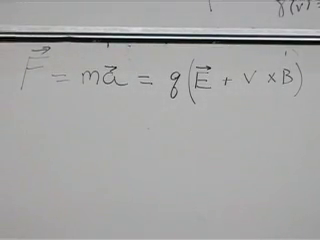
\includegraphics[width=0.8\textwidth]{lecture_06_figure_06.png}
\caption{\(\boldsymbol E\)と\(\boldsymbol B\)を組み合わせる動機となる、相対論以前の形のローレンツ力の法則。}
\lectureframe{01:18:20}
\end{figure}

ある観測者が電場を見ずに磁場と運動する電荷を見ているとしよう。その電荷は磁気的な力を受ける。しかし、その電荷の瞬間静止系では\(\boldsymbol v=0\)であるから、式~\eqref{eq:l6-lorentz-force}の磁気の項は消える。座標が変わったからといって物理的な世界線が慣性になっているわけではない。したがって、新しい系における力には電気的な寄与が含まれなければならない。より注意深く言えば、非零の四元加速度は、慣性系を変えても零に変換することはできない。ただし、三次元加速度とその成分は変換される。\editorialnote{この四元加速度についての主張は、教室での議論の不変形であり、通常の三次元加速度そのものを系に不変なものとして扱うことを避けている。}

したがって、電場と磁場は互いに変換し合わなければならない。両者を合わせると六つの成分をもつので、一つのスカラーでも一つの四元ベクトルでもない。新たな変換する対象が必要である。

\section{テンソル：各添字に一つの変換}

スカラーは階数零のテンソルと呼ばれることがある。添字をもたない。四元ベクトルは階数一のテンソルであり、四つの可能な値をもつ添字を一つもつ。最も簡単な階数二の例は積
\begin{equation}
  A^\mu B^\nu.
\end{equation}
である。各添字が四つの値をとるので、この対象は\(4^2=16\)個の成分をもち、\(4\times4\)の配列として表示できる。三つのベクトルの積
\begin{equation}
  A^\mu B^\nu C^\sigma,
\end{equation}
は\(4^3=64\)個の成分をもち、階数三のテンソルである。より高い階数もこのパターンに従う。名称よりも、その対象を定義する規則の方が重要である。

もし
\begin{equation}
  A'^{\mu}=\Lambda^\mu{}_{\nu}A^\nu,
  \qquad
  B'^{\sigma}=\Lambda^\sigma{}_{\tau}B^\tau,
\end{equation}
ならば、それらの積は
\begin{equation}
  A'^{\mu}B'^{\sigma}
  =\Lambda^\mu{}_{\nu}\Lambda^\sigma{}_{\tau}
   A^\nu B^\tau.
\end{equation}
と変換する。これにより、反変階数二テンソルの定義則が与えられる：
\begin{equation}
  T'^{\mu\sigma}
  =\Lambda^\mu{}_{\nu}\Lambda^\sigma{}_{\tau}T^{\nu\tau}.
                                                                  \label{eq:l6-tensor-transform}
\end{equation}
各添字に対して一つのローレンツ行列がある。繰り返された\(\nu\)と\(\tau\)は和をとられ、開いた\(\mu\)と\(\sigma\)はプライム系で計算される成分を表す。

\begin{figure}[H]
\centering
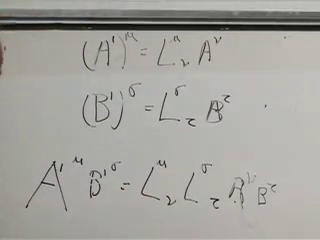
\includegraphics[width=0.82\textwidth]{lecture_06_figure_07.png}
\caption{二つのベクトルの変換と、それから得られる階数二テンソルの二行列変換則。}
\lectureframe{01:27:15}
\end{figure}

テンソルはベクトルの単一の積である必要はない。\(A^\mu B^\nu\)も\(A^\nu B^\mu\)もテンソル変換則を満たし、それらの和や
\begin{equation}
  A^\mu B^\nu+C^\mu D^\nu.
\end{equation}
のような任意の和も同様である。定義となるのは変換則であり、特定の因数分解ではない。階数三のテンソルは三つ目のローレンツ行列を獲得し、以下同様である。

\section{対称テンソルと反対称テンソル}

階数二のテンソルのうち二つのクラスが特に有用である。対称テンソルは
\begin{equation}
  T^{\mu\nu}=T^{\nu\mu},
\end{equation}
を満たすので、対角線を挟んで反射した成分は一致する。四つの対角成分と対角線の片側にある六つの成分が残りを決定し、\begin{equation}
  4+6=10
\end{equation}
個の独立成分を与える。

反対称テンソルは
\begin{equation}
  T^{\mu\nu}=-T^{\nu\mu}.                                \label{eq:l6-antisymmetry}
\end{equation}
を満たす。式~\eqref{eq:l6-antisymmetry}で\(\mu=\nu\)と置くと
\(T^{\mu\mu}=-T^{\mu\mu}\)となるので、すべての対角成分は消える。一方の三角形の半分にある六つの成分が、符号を変えることでもう六つを決定する。したがって、独立成分はちょうど六つである。

\begin{figure}[H]
\centering
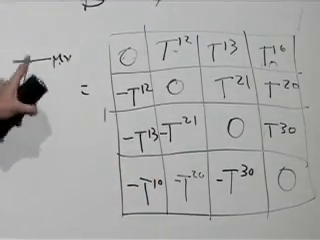
\includegraphics[width=0.82\textwidth]{lecture_06_figure_08.png}
\caption{完成した反対称\(4\times4\)配列：対角線上は零で、対角線を挟んで符号が反対。}
\lectureframe{01:34:25}
\end{figure}

この数が手がかりである。三つの電場成分と三つの磁場成分は、一つの反対称階数二テンソルに収めることができる。

\section{電磁場テンソル}

時空のラベルが\((1,2,3,0)=(x,y,z,t)\)の順で行と列に並ぶとしよう。黒板に書かれた配置は
\begin{equation}
  F_{\mu\nu}=
  \begin{pmatrix}
    0    & -B_3 & B_2  & E_1\\
    B_3  & 0    & -B_1 & E_2\\
    -B_2 & B_1  & 0    & E_3\\
    -E_1 & -E_2 & -E_3 & 0
  \end{pmatrix}.                                         \label{eq:l6-field-tensor}
\end{equation}
である。純粋に空間的な位置には磁場が入り、一つの空間添字と一つの時間添字をもつ位置には電場が入る。反対称性により、上三角成分が分かれば下三角成分が与えられる。

\begin{classroomqa}
\audiencequestion{磁気の成分はすべて負であり、ラベルは\(x,y,z\)に対応するのか。}
\lecturerresponse{上側の空間三角形における符号は示されたように交互になる：\(-B_3,+B_2,-B_1\)。ラベル\(1,2,3\)は\(x,y,z\)に対応し、一方\(0\)は時間を表す。対角線を挟んだ反射はすべての符号を逆にする。}
\end{classroomqa}

\begin{figure}[H]
\centering
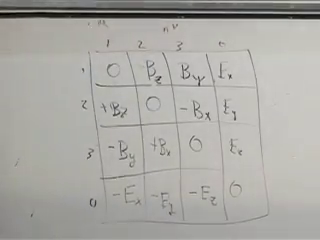
\includegraphics[width=0.82\textwidth]{lecture_06_figure_09.png}
\caption{講義の空間優先の成分順序における、完成した電磁場テンソル。}
\lectureframe{01:41:05}
\end{figure}

この記法は慣例的に\(F_{\mu\nu}\)であり、一般的な\(T_{\mu\nu}\)ではない。講師は、この文字はFaradayを指すのではないかと推測しつつも、この記法の歴史については知らないと明言している。ここで重要なのは、この文字についてのその推測ではなく、その反対称性と6つの場の成分である。

\begin{classroomqa}
\audiencequestion{各行列成分は、示された座標平面における場の強さを表しているのか。}
\lecturerresponse{それは電磁場テンソルの成分である。時間を含む成分は電場成分であり、空間--空間の成分は磁場成分を表す。}
\end{classroomqa}

時間指数をもつ行と列を切り分ける。残る\(3\times3\)の反対称ブロックが磁場である。その独立な成分は巡回的に覚えられる：
\begin{equation}
  F_{12}=-B_3,
  \qquad F_{23}=-B_1,
  \qquad F_{31}=-B_2.                                   \label{eq:l6-magnetic-cycle}
\end{equation}
最初の関係から出発し、すべてのラベルを\(1\to2\to3\to1\)に沿って進める。等価的には、
\begin{equation}
  F_{ij}=-\epsilon_{ijk}B_k,
\end{equation}
ただし\(\epsilon_{123}=+1\)とする。\editorialnote{Levi--Civitaの公式は、黒板で明示的に展開された巡回規則の簡潔な標準形である。}

\begin{figure}[H]
\centering
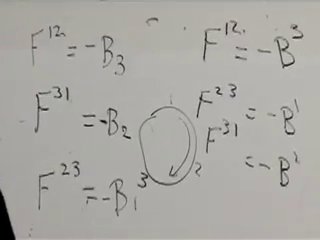
\includegraphics[width=0.82\textwidth]{lecture_06_figure_10.png}
\caption{反対称テンソルにおいて磁場を表す巡回的な空間成分。}
\lectureframe{01:46:20}
\end{figure}

電場の同定はより直接的である：
\begin{equation}
  E_1=F_{10},
  \qquad E_2=F_{20},
  \qquad E_3=F_{30}.
\end{equation}

したがって磁場には2つの有用な同一視がある。3次元空間内では、3成分の軸性ベクトルを\(3\times3\)の反対称テンソルと対応させることができる。しかし時空では、それは6成分テンソル\(F_{\mu\nu}\)の空間部分にすぎない。この対応は3次元に特有である：反対称な\(4\times4\)テンソルは6つの独立な成分をもち、4元ベクトルと同一視することはできない。\editorialnote{固有回転の下で磁場はベクトルとして振る舞うが、反射の下ではより正確には軸性ベクトル、すなわち擬ベクトルである。}

この構成の目的は、成分を数えること自体ではない。\(F_{\mu\nu}\)がテンソルとして変換するため、ローレンツブーストは自動的にその電場成分と磁場成分を混合する。次の講義では、これを4元速度および4元加速度と組み合わせて、式~\eqref{eq:l6-lorentz-force}を共変な運動方程式に置き換えることができる。

\section{EinsteinとMinkowskiに関する質問}

最後の数分は、形式論からそれが歴史的にどのように生じたかに移る。答えは確定した歴史ではなく回想として述べられ、その留保はこのやり取りの一部である。

\begin{classroomqa}
\audiencequestion{Einsteinは概念的根拠からローレンツ不変な定式化を求めていたのか、それとも特定の観測に突き動かされていたのか。}
\lecturerresponse{自然法則はすべての慣性系で同じ形をとるべきであるという原理が、彼の推論の中心にあった。光に関する実験的証拠や、エーテルを通る運動が検出されなかったこともあったが、講師は、Einsteinがどの結果を知っていたのか、あるいはそれらがどれほど強く彼に影響したのかについては明示的に不確かであると述べている。概念的圧力は、Maxwell方程式とローレンツ力が相対性原理に従うべきであり、それには電場、磁場、速度成分がともに変換することが要求されるという点にあった。}
\end{classroomqa}

Einsteinの1905年の発表は、ここで用いられている簡潔な4元ベクトル記法を使っていなかった。それは成分ごとに進められ、必要な\(\gamma\)の因子と速度が明示的に書かれていた。その後Minkowskiが、同じ構造を4次元時空として幾何学的に整理した。

\begin{classroomqa}
\audiencequestion{EinsteinはMinkowskiの時空定式化に抵抗したのか、またMinkowskiはどれほど早くそれを導入したのか。}
\lecturerresponse{授業で述べられた回想によれば、Einsteinは当初4次元幾何学的言語を歓迎しなかったが、その価値をすぐに取り入れた。時期は、1905年の論文のおよそ2年後、おそらく1907年ごろと暫定的に示され、話し手は、歴史を確定しているのではなく回想しているのだと強調する。}
\end{classroomqa}

\begin{classroomqa}
\audiencequestion{Minkowskiは数学者だったのか物理学者だったのか、他に何に貢献したのか、またLorentzやFitzGeraldの影響を受けたのか。}
\lecturerresponse{確信をもった答えは主張されない。数学者と物理学者の区別は追及されず、Minkowskiの他の仕事についての広い発言は聴衆からの訂正によって中断され、影響の可能性のある筋道は明示的に不確かなままにされる。この議論にとって確かな点は、Minkowskiが相対性理論を4次元幾何学的記法で決定的に整理したことである。}
\end{classroomqa}

\begin{classroomqa}
\audiencequestion{\(\boldsymbol E\)と\(\boldsymbol B\)を混合する変換は、すでにアインシュタインの1905年の仕事に存在していたのであろうか。}
\lecturerresponse{はい、しかし一つの場のテンソル方程式としてではなく、成分ごとに書かれていた。授業で行った比較はマクスウェルの成分方程式との比較である。内容は、その共通構造を明らかにする簡潔な記法より前に存在しうる。ミンコフスキーの貢献は、その構造を時空の言葉で体系的にしたことであった。}
\end{classroomqa}

これで、我々が出発点とした数学的な論点に戻る。成分は計算には不可欠であるが、それらの成分が一つの変換する対象の部分であると認識されるとき、法則は理解可能になる。次の課題は、\(F_{\mu\nu}\)を用いて、荷電粒子の運動方程式を、すべての慣性系で同じ形になるように書くことである。
